\documentclass[conf]{new-aiaa}
%\documentclass[journal]{new-aiaa} for journal papers
\usepackage[utf8]{inputenc}

\usepackage{graphicx}
\usepackage{amsmath}
\usepackage{commath}
\usepackage[version=4]{mhchem}
\usepackage{siunitx}
\usepackage{longtable,tabularx}
\usepackage{float}
\usepackage{listings}
\usepackage{color} %red, green, blue, yellow, cyan, magenta, black, white
\definecolor{mygreen}{RGB}{28,172,0} % color values Red, Green, Blue
\definecolor{mylilas}{RGB}{170,55,241}
\setlength\LTleft{0pt} 

\lstset{language=Matlab,%
	basicstyle=\footnotesize,
	breaklines=true,%
	morekeywords={matlab2tikz},
	keywordstyle=\color{blue},%
	morekeywords=[2]{1}, keywordstyle=[2]{\color{black}},
	identifierstyle=\color{black},%
	stringstyle=\color{mylilas},
	commentstyle=\color{mygreen},%
	showstringspaces=false,%without this there will be a symbol in the places where there is a space
	numbers=left,%
	numberstyle={\tiny \color{black}},% size of the numbers
	numbersep=9pt, % this defines how far the numbers are from the text
	emph=[1]{for,end,break},emphstyle=[1]\color{red}, %some words to emphasise
	%emph=[2]{word1,word2}, emphstyle=[2]{style},    
}

% ================================================================ % 
\title{ASE 389P.4 Methods of Orbit Determination \\ Homework 2: Orbit Propagation with Perturbations}

\author{Junette Hsin}
\affil{Masters Student, Aerospace Engineering and Engineering Mechanics, University of Texas, Austin, TX 78712}

\begin{document}

\maketitle

\begin{abstract}
New force models have been added to the orbit propagator created in Homework 1. The effects that these new forces have on the Keplerian orbit elements and the
total specific energy were analyzed.

\end{abstract}


% ================================================================ % 
\section{Introduction}

%HW1 intro: In this assignment, a tool was created to numerically propagate a circular orbit about the Earth and to convert between Cartesian and Keplerian orbital elements. 2 solutions for the derivation of the gradient potential function are given. 2-body equations of motion and constants of motion are also explored. The software implemented in this assignment will be used later in the course provides additional background and/or a review of basic orbital mechanics.


% ================================================================ % 
\section{Problem 1}

\subsubsection{Statement} 
\begin{center}
\fbox{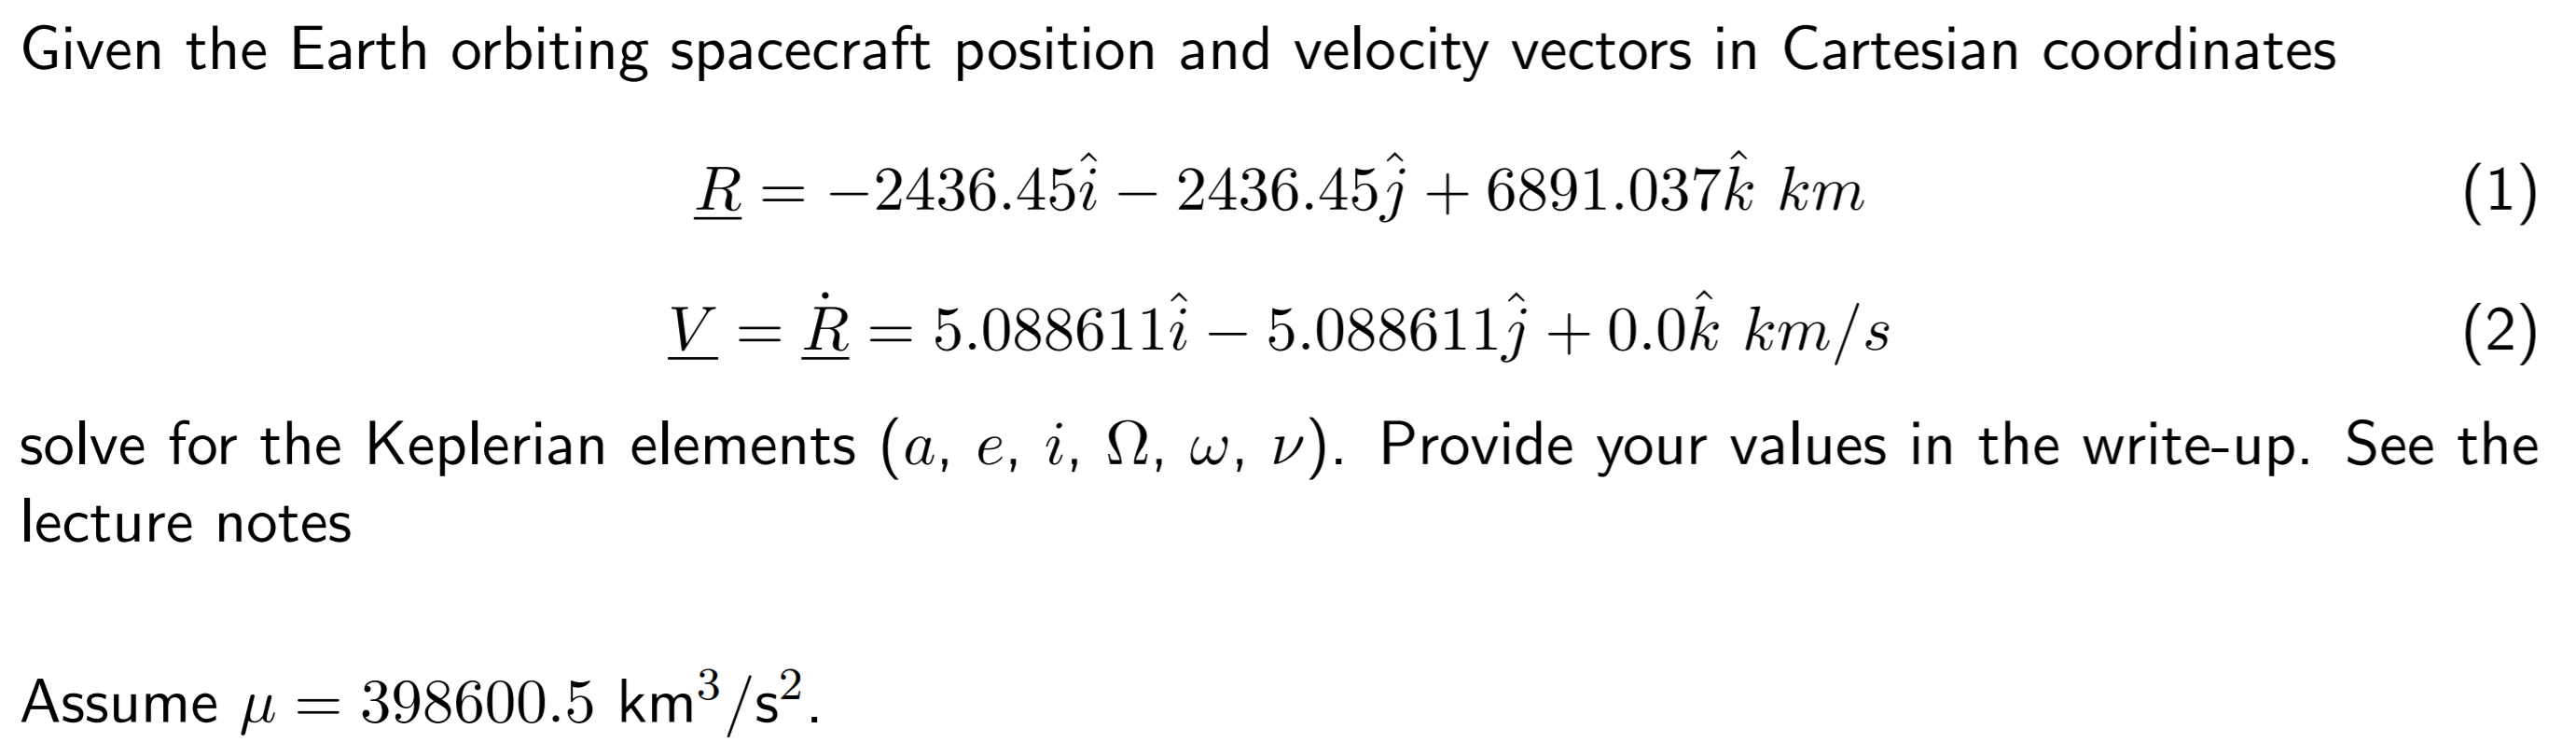
\includegraphics[width=0.9\textwidth]{prob_1.png}} \\
\end{center}

% ---------------------------------------------------------------- % 
\subsubsection{Solution} 

%The algorithms to convert orbital elements to Cartesian and back were taken from References \cite{bate_astrodynamics} and \cite{jah_mod3}. First, the specific angular momentum vector, $h$, and perpendicular node vector (to the plane of the orbit), $n$, were calculated. Inclination, eccentricity, and the rest of the orbital elements followed while checking for equatorial orbits, NaNs, and quadrants of angles. Given the spacecraft position and velocity vectors from the problem statement, the Keplerian elements are: 
%
%\begin{equation}
%\begin{aligned}
%a = &~ 7.712184983762814e+03 \\ 
%e = &~ 0.447229247404423 \\ 
%i = &~ 1.570796326794897 \\ 
%\omega = &~ 3.139593866862924 \\ 
%\Omega = &~ 3.926990816987241 \\ 
%\nu = &~ 2.032461649676350  
%\end{aligned}
%\end{equation}
%
%where $a$ is the semi-major axis, $e$ is the eccentricity, $i$ is the orbit inclination, $\omega$ is the argument of perigee, $\Omega$ is the right ascension of the ascending node, and $\nu$ is the true anomaly. 


% ================================================================ % 

\subsection{Problem 1a} 
\begin{center}
	\fbox{
\includegraphics[width=0.9\textwidth]{prob_2.png}} \\
\end{center}

\subsubsection{Statement} 

% ---------------------------------------------------------------- % 

\subsubsection{Solution} 


% ================================================================ % 

\subsection{Problem 1b} 
\begin{center}
	\fbox{
\includegraphics[width=0.9\textwidth]{prob_2.png}} \\
\end{center}

\subsubsection{Statement} 

% ---------------------------------------------------------------- % 

\subsubsection{Solution} 



% ================================================================ % 

\subsection{Problem 1c} 
\begin{center}
	\fbox{
\includegraphics[width=0.9\textwidth]{prob_2.png}} \\
\end{center}

\subsubsection{Statement} 

% ---------------------------------------------------------------- % 

\subsubsection{Solution} 




% ================================================================ % 

\subsection{Problem 1d} 
\begin{center}
	\fbox{
\includegraphics[width=0.9\textwidth]{prob_2.png}} \\
\end{center}

\subsubsection{Statement} 

% ---------------------------------------------------------------- % 

\subsubsection{Solution} 


% ================================================================ % 

\section{Conclusion} 

%HW1: Calculating orbital elements to and from Cartesian position and velocity vectors can be tricky because of the quadrant ambiguities when performing trigonometric computations. Problem 3 might have included a typo in its problem statement for the gravity potential function; the potential is commonly given as $U = \mu/r$ in which r is the distance between 2 bodies, not $U = \mu / ( \underline{R} \cdot \underline{R} )$. Solutions were given for both potential equations. Though position and velocity may vary along an orbit, there are constants of motion such as angular momentum and specific mechanical energy which govern the motion of celestial bodies. 



% ================================================================ % 

\newpage
\section{Appendix} 

\subsection{HW1 MATLAB code} 

\begin{lstlisting}[basicstyle=\footnotesize]
% ASE 389 Orbit Determination
% HW 1
% Junette Hsin 

%% Problem 1 

global mu 

mu = 398600.5 ; 
r  = [ -2436.45; -2436.45; 6891.037 ]; 
v  = [ 5.088611; 5.088611; 0 ]; 

rv = [r; v]; 
oe = rv2oe(rv);  

%% Problem 2 

rv = oe2rv(oe); 

%% Problem 3 

x = -2436.45; 
y = -2436.45; 
z = 6891.037; 
mu = 398600.5; 

dux = -2*mu*x / ( x^2 + y^2 + z^2 )^2; 
duy = -2*mu*y / ( x^2 + y^2 + z^2 )^2;
duz = -2*mu*z / ( x^2 + y^2 + z^2 )^2;

rnorm = sqrt( x^2 + y^2 + z^2 ); 

dux = -mu*x / ( rnorm )^3; 
duy = -mu*y / ( rnorm )^3; 
duz = -mu*z / ( rnorm )^3;

%% Problem 4 

a = oe(1); 
T   = abs(2 * pi * sqrt(a^3 / mu));        % period 

toler   = 1e-8;         % 1e-14 accurate; 1e-6 coarse 
options = odeset('reltol', toler, 'abstol', toler ); 
[t,x] = ode45(@TwoBod_6states, [0 2*T], [r; v], options); 

for i = 1:length(t)
rnorm(i) = norm(x(i, 1:3)); 
vnorm(i) = norm(x(i, 4:6)); 
H(i, :) = cross(x(i, 1:3), x(i, 4:6)); 
hnorm(i) = norm(H(i, :)); 
end 

anorm = 0; 
for i = 2:length(t)
a = (x(i, 4:6) - x(i-1, 4:6)) / ( t(i) - t(i-1) ); 
anorm(i) = norm(a); 
end 

% ------------------------------------------------------------------------

name = 'Problem 4: 2-Body EOM'; 
h = figure('name', name); 

% position 
subplot(3,1,1)
plot(t, rnorm); grid on 
title('r norm') 
ylabel('km')

% velocity 
subplot(3,1,2) 
plot(t, vnorm); grid on 
title('v norm') 
ylabel('km/s')

% acceleration 
subplot(3,1,3) 
plot(t, anorm); grid on 
title('a norm'); 
ylabel('km/s^2')
xlabel('time (sec)') 

sgtitle(name)

save_pdf(h, 'prob4_2bodeom'); 

% ------------------------------------------------------------------------

name = 'Problem 4: 2-Body EOM Orbit'; 
h = figure('name', name); 
plot3(x(:,1), x(:,2), x(:,3)); hold on; grid on; 
plot3(x(1,1), x(1,2), x(1,3), 'o')
plot3(x(end,1), x(end,2), x(end,3), 'x') 
xlabel('x (km)')
ylabel('y (km)') 
zlabel('z (km)') 
legend('orbit', 'start', 'end')

sgtitle(name) 

save_pdf(h, 'prob4_2bodeom_orbit'); 

% ------------------------------------------------------------------------

clear oe 
for i = 1:length(t)
oe(i,:) = rv2oe(x(i,:)); 
end 

labels = {'a', 'e', 'i', '\omega', '\Omega', '\nu'}; 
units = {'km', '', 'rad', 'rad', 'rad', 'rad'}; 
name = 'Problem 4: 2-Body Orbital Elements'; 
h = figure('name', name, 'position', [100 100 500 600]); 
for i = 1:6
subplot(6,1,i)
plot(t, oe(:, i)); grid on 
title(labels{i}); 
ylabel(units{i}); 
end 
xlabel('time (sec)') 
sgtitle(name)

save_pdf(h, 'prob4_2bodoes'); 

% ------------------------------------------------------------------------

name = 'Problem 4: 2-Body Specific Angular Momentum'; 
h = figure('name', name); 
subplot(2,1,1) 
scatter3(H(:,1), H(:,2), H(:,3)); grid on 
xlabel('x (km^2/s)')
ylabel('y (km^2/s)')
zlabel('z (km^2/s)') 
title('h (scatter plot)') 

subplot(2,1,2) 
plot(t, hnorm); grid on 
xlabel('time (sec)') 
ylabel('km^2/s') 
title('h norm vs time')

sgtitle(name) 

save_pdf(h, 'prob4_angmom')

%% Problem 5 

% specific kinetic energy 
for i = 1:length(t) 
T(i) = 0.5 * vnorm(i)^2; 
U(i) = mu / rnorm(i); 
end 
E = T - U; 

name = 'Problem 4: 2-Body Specific Energy'; 
h = figure('name', name); 
subplot(2,1,1) 
plot(t, E); grid on; hold on; 
plot(t, T); 
plot(t, U); 
ylabel('km^2/s^2')
legend('Total', 'Kinetic', 'Potential') 
title('Total Specific Energy: Kinetic - Potential') 
subplot(2,1,2) 
plot(t, [0 diff(E)]); grid on 
title('Change in Total Specific Energy') 
xlabel('Time (sec)') 
ylabel('km^2/s^2')
sgtitle(name) 

save_pdf(h, 'prob5_energy')

%% subfunctions 

function save_pdf(h, name) 

% save as cropped pdf 
set(h,'Units','Inches');
pos = get(h,'Position');
set(h,'PaperPositionMode','Auto','PaperUnits','Inches','PaperSize',[pos(3), pos(4)])
print(h,name,'-dpdf','-r0')

end 
\end{lstlisting}

\subsection{rv2oe function}

\begin{lstlisting}[basicstyle=\footnotesize]
function oe = rv2oe(rv)
% ------------------------------------------------------------------------
% Inputs 
%   rv = [6x1] position and velocity states vector 
% 
% Outputs 
%   oe = [6x1] orbital elements: a, e, i, w, Omega, nu
%           a       = semimajor axis 
%           e       = eccentricity 
%           i       = inclination 
%           w       = argument of perigee 
%           Omega   = right ascension of ascending node 
%           nu      = true anomaly 
% ------------------------------------------------------------------------

global mu 

r = rv(1:3); 
v = rv(4:6); 

% angular momentum 
h       = cross(r,v); 

% node vector 
nhat    = cross( [0 0 1], h ); 

% eccentricity 
evec    = ( (norm(v)^2 - mu/norm(r))*r - dot(r,v)*v ) / mu; 
e       = norm(evec); 

% specific mechanical energy 
energy  = norm(v)^2/2 - mu/norm(r); 

% semi-major axis and p
if abs(e-1.0)>eps
a = -mu/(2*energy); 
p = a*(1-e^2); 
else
p = norm(h)^2/mu; 
a = inf; 
end

% inclination 
i = acos(h(3)/norm(h)); 

% right ascension of ascending node (check for equatorial orbit) 
if i > 0.000001
Omega = acos( nhat(1)/norm(nhat) ); 
else
Omega = 0; 
end
if isnan(Omega)
Omega = 0; 
end
if nhat(2)<0
Omega = 2*pi - Omega; 
end

% argument of perigee 
if e > 0.000001
w = acos(dot(nhat,evec)/(norm(nhat)*e)); 
else
w = 0; 
end
if isnan(w)
w = 0; 
end
% if e(3)<0
%    argp = 360-argp
% end

% true anomaly 
nu = acos( dot(evec,r) / (e*norm(r)) );  
% if dot(r,v)<0
%    nu = 360 - nu
% end

oe = [a; e; i; w; Omega; nu]; 

end
\end{lstlisting}

\subsection{oe2rv function}

\begin{lstlisting}
function [rv] = oe2rv(oe)
% ------------------------------------------------------------------------ 
% Purpose: Convert orbital elements and time past epoch to the classic 
% Cartesian position and velocity
% 
% Inputs: 
%   oe      = [6x1] or [1x6] orbital elements 
%   delta_t = t - t0 time interval 
%   mu      = Gravity * Mass (of Earth) constant 
% 
% Outputs: 
%   rv      = position and velocity state vector 
% ------------------------------------------------------------------------ 

% global delta_t 
global mu 

a       = oe(1); 
e       = oe(2); 
i       = oe(3); 
w       = oe(4); 
LAN     = oe(5); 
% M0      = oe(6); 
nu      = oe(6); 

% nu is TRUE ANOMALY --> use Kepler's to calculate MEAN ANOMALY 
% E = 2*atan( sqrt( (1-e)/(1+e) ) * tan(nu/2) ); 
% M = M0 + sqrt( mu/a^3 ) * (delta_t); 
% E = keplerEq(M, e, eps); 
% E = kepler(M, e); 
% nu = 2*atan( sqrt( (1+e)/(1-e) ) * tan(E/2) ); 

p = a * ( 1 - e^2 );            % intermediate variable 
r = p / ( 1 + e*cos(nu) );      % r_magnitude, polar coordinates 

% Perifocal position and velocity 

r_pf = [ r * cos(nu); r * sin(nu); 0 ]; 
v_pf = [ -sqrt(mu/p) * sin(nu); sqrt(mu/p) * (e + cos(nu)); 0 ]; 

% Perifocal to ECI transformation, 3-1-3 rotation 
R11 = cos(LAN)*cos(w) - sin(LAN)*sin(w)*cos(i); 
R12 = -cos(LAN)*sin(w) - sin(LAN)*cos(w)*cos(i); 
R13 = sin(LAN)*sin(i); 

R21 = sin(LAN)*cos(w) + cos(LAN)*sin(w)*cos(i); 
R22 = -sin(LAN)*sin(w) + cos(LAN)*cos(w)*cos(i); 
R23 = -cos(LAN)*sin(i); 

R31 = sin(w)*sin(i); 
R32 = cos(w)*sin(i); 
R33 = cos(i); 

R = [R11 R12 R13; R21 R22 R23; R31 R32 R33]; 

% Transform perifocal to ECI frame 
r_vec = R * r_pf; 
v_vec = R * v_pf; 

% Position and state vector 
rv = [r_vec; v_vec]; 

end 

%% Kepler equation solvers 

function E = keplerEq(M,e,eps)
% Function solves Kepler's equation M = E-e*sin(E)
% Input - Mean anomaly M [rad] , Eccentricity e and Epsilon 
% Output  eccentric anomaly E [rad]. 
En  = M;
Ens = En - (En-e*sin(En)- M)/(1 - e*cos(En));
while ( abs(Ens-En) > eps )
En = Ens;
Ens = En - (En - e*sin(En) - M)/(1 - e*cos(En));
end
E = Ens;
end

function E = kepler(M, e)
f = @(E) E - e * sin(E) - M;
E = fzero(f, M);  % <-- I would use M as the initial guess instead of 0
end
\end{lstlisting}

% ================================================================ % 

s\bibliography{sample}

\end{document}
